The problem of antrhopomorphizing machine learning applications is that, often, 
those statements come from marketing departments or reporters who've ever trained 
a model. They haven't realized (or deliberately omit) an obvious flaw that all 
the algorithms and techniques share in practice: \textbf{they don't train, they 
are trained by humans.}

Actually, there is an incredibly ammount of human work in every machine learning 
project that comes from human labour, including: 

\begin{itemize}
	\item \textbf{Data preparation:} every model has his own requirements about 
		data format. 
	\item \textbf{Data cleansing:} most algorithms assume that their training 
		phase will be conducted over a perfectly curated data set: \textit{
		zip codes that actually refer geographical information, missing data 
		to be imputed...}
	\item \textbf{Context awareness:} That's specially important in the case 
		of neural networks. Way before running the first epoch, the researcher 
		or data scientist, must figure out how to express problem's logic in a 
		language that the network can deal with. Sometimes this represent a 
		straightforward requirement, sometimes is nearly impossible. 
	\item \textbf{Disambiguation, cultural biases:} Machine learning inherits \cite{gorilla}
		all sort of biases included in the training dataset. It's human responsability 
		to prune them.  
\end{itemize}

Event thought their inherent difficulty and prevalence, the aforementioned arguments 
could be considered \textit{low-level} tasks in the context of artificial 
intelligence. Not a real concern for the \textit{singularity} concept.

Specially if we assume Kurzweil's full thesis, i.e., that the singularity will 
reach by a mixed human and artificial intelligence. What he called \textit{human 
2.0} would be a human body empowered with the benefits of the kind of \textit{
learning} we associate with current machine learning or deep learning systems.

On the one hand, this scenario would overcome all the problems mentioned until now: 
the human brain will still be there to manage them. But, in the other hand, all what w
we did adopting the \textit{human 2.0} argument is changing the perspective. Now 
the questions look different.

\textbf{How reliable this brand new learning is?}

Sadly, in practice, even slightly departures from the nature of training data could
turn the finest tuned models into completely absurd predictors.

Recent research on "adversarial examples"\cite{adversarial} has shown how adding 
noise (inperceptible to human eye) to well classified images can substantially modify 
the output.

\begin{figure}[h!]
	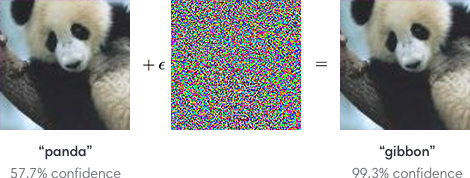
\includegraphics[width=\linewidth]{images/panda.png} % Figure image
	\caption{Adding noise ruin the predictions} % Figure caption
	\label{bear} % Label for referencing with \ref{bear}
\end{figure}

The system starts, suddenly, saying that panda bears are gibbons; \cite{panda} or refuses to 
recognize image's contents depending on the process followed to capture them.

\textbf{Deep learners, learn. But they don't understand.}

\textbf{You want me to become a cyborg, right? Does it worth? Will it add 
something fundamentally valuable to my current intelectual toolbox?}

Regarding this question (which, basically, inquires on what are the theoretical 
limitations of machine learning) we should consider John Lauchbury's \textit{
"manifold hypothesis"} \cite{darpa} 

In short, this hypothesis states a generalization to a high-dimensional space 
of the well-known linear separability problem. Where a simple perceptron isn't 
able to \textit{learn} a non-linearly separable group of clusters in a given 
dataset; the extension to multidimensional spaces considers that clusters adopt 
the form of manifolds and entangled manifolds that cannot be separated produce 
datasets that cannot be learned.

This geometric stance links the problem of deciding when culstering (or 
"classification" or "learning") can be performed over a general dataset with 
the mathematical field of topological manifolds, particularly with the question 
of entangled manifolds separability.\cite{topology}

Both questions lack from a general answer. But the adoption of this \textit{
geometrical} view fills one important gap in some machine learning (deep or not) 
setups: the explainability of the models after training.

Lookgin through the topology glass, neural networks have only one job: to perform 
continuous transformations between spaces. 

	\begin{figure}[h!]
\begin{center}
		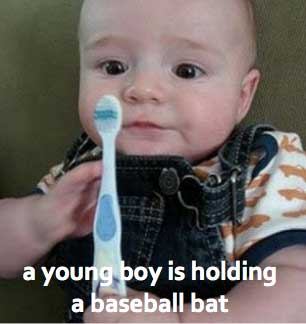
\includegraphics[height=5cm]{images/baby.jpg} % Figure image
		\caption{Artificially generated caption: toothbrush $=$ bat} % Figure caption
		\label{baby} % Label for referencing with \ref{bear}
\end{center}
	\end{figure}

And humans are overwhelmingly good at it. That's why we'd never confuse a bat 
with a toothbrush.  
